\section{The PGAC detectors}
\subsection{Introduction}
The TRIUMF Detector Group has developed the EMMA PGAC (Parallel Grid Avalanche Counter), a device that is designed to work with the radioactive beams delivered by ISAC-II at TRIUMF.  The PGAC detector will be a key component of the detector suite at the focal plane of the EMMA spectrometer.
EMMA, currently under construction in ISAC-II,  is a recoil mass spectrometer 
which %uses electric and magnetic dipoles to
 separates recoils of nuclear reactions from the accelerated ion beam.  The reaction recoils and the unreacted beam will be dispersed  according to their mass/charge ratio.  By separating beam-like recoils from the unreacted beam, very weak reaction channels may be studied in the presence of very high-yield background channels.  In a similar manner, beam contaminants may also be separated.  Ultimately the PGAC will form the entrance to the EMMA ionization chamber, a large-acceptance Bragg detector which will be used to provide $Z$-identification of the  recoils.

 %Some of the relevant specifications of the detector are listed in Table~\ref{detector}.
The EMMA PGAC is designed to measure the position of particles in the $x$-$y$ plane at the EMMA focal plane. %The PGAC will also provide an essential timing signal for EMMA experiments.
  The timing reference provided by the PGAC is used to measure the recoil time-of-flight, the recoil coincidence with ejectiles detected in the target chamber, and is used to generate the trigger for the data acquisition system. 
Two identical PGACs have been constructed and both were tested simultaneously in a purpose-built test chamber.  The purpose of the test was to characterize the detectors and determine their position and time resolution.

\subsection{Principle of Operation}
The EMMA PGAC is a position-sensitive, multi-wire, gas-filled proportional counter optimized for the detection of heavy ions.  The PGAC is filled with isobutane at a nominal pressure of $P=2$--6\,Torr.\footnotemark[3] %
\footnotetext[3]{Further information regarding the use of isobutane can be found in the EMMA PGAC Detector Test Safety Report: \newline  \textit{\hspace*{1.5em}}
\url{https://documents.triumf.ca/docushare/dsweb/Get/Document-109474/PGAC_safety.pdf}}%
The detector consists of three electrode planes: a cathode that is position sensitive in the $y$-direction; an anode; and a cathode that is position sensitive in the $x$-direction.  The anode is centered between the two cathodes.  Each electrode consists of a plane of parallel wires.

Heavy ions passing through the gas volume of the detector will cause ionization that will be accelerated by the %high
 voltages applied to the electrodes.  The motion of the ionized gas particles in the electric field produces secondary ionization in the gas, thus multiplying the initial ionization into an ion avalanche.
The  voltage applied to the anode and cathode depend on the operating pressure of the detector.  At $P=4$\,Torr, the voltage difference between the anode and cathode is typically $\Delta V=550$\,V.  The anode is held at a positive voltage, $V_\textrm{a}=470$\,V at $P=4$\,Torr.  The two cathodes are held at a relatively small negative voltage, $V_\textrm{c}=-80$\,V at $P=4$\,Torr.  The negative voltage on the cathodes is used to produce a potential difference between the cathodes and the walls of the chamber, which are at ground potential, in order to prevent the detection of ionization from outside of the active region.  

For each event, seven signals are output by each PGAC. Each cathode has two output signals that are used to derive a position.  One cathode measures positions in the $x$-direction, the other measures positions in the $y$-direction, for a total of four cathode signals.  The anode is divided into three sections to reduce the capacitance of the detector and improve timing performance.  The anode signal is the characteristic timing signal of the PGAC.% and it 


\subsection{Technical Description}
The PGAC detectors are shown in Fig.~\ref{wire_planes}.
The general properties of the detectors are summarized in Table~\ref{detector_specs}  
The PGAC detectors are rectangular in cross section with %an active 
an open area of 166\,mm in the $x$-direction and 66\,mm in the $y$-direction.  
As shown in Fig.~\ref{wire_planes}\,(Left), each detector consists of a stack of three printed circuit boards (PCB).  Each PCB supports a wire plane.  The wire planes of each detector are separated by 1/8\,in or 3.18\,mm and are arranged such that the anode is centered between the two cathodes.

\begin{table}[ht!]
\begin{center}
\begin{tabulary}{1.0\textwidth}{R|L} 
%\begin{tabular}{p{0.45\columnwidth}|p{0.45\columnwidth}} 
\raggedleft Gas (ionization media)&Isobutane\\
\raggedleft Nominal operating pressure range&$P=2$--6\,Torr\\
\hline
\raggedleft Window material &Mylar\\
\raggedleft Nominal window thickness&1--2\,$\mu$m\\
\raggedleft Window area& 66\,mm $\times$ 166\,mm (110\,cm$^2$)\\
\raggedleft Window position (from anode)& $-36.3$\,mm\hspace{5.4em}(test)\\
&$-27.2$\,mm,  $+52.8$\,mm (focal plane)\\
\hline
\raggedleft Wire material&Gold-plated tungsten\\
\raggedleft Cathode wire diameter&25\,$\mu$m\\
\raggedleft Cathode wire pitch&1.0\,mm\\
\raggedleft Number of cathode wires&166 ($x$-direction)\\
& ~~66 ($y$-direction)\\
\raggedleft Anode wire diameter&15\,$\mu$m\\
\raggedleft Anode wire pitch&1.0\,mm\\
\raggedleft Number of anode wires &$3\times22$\\  
\raggedleft Anode-cathode gap&3.18\,mm\\
\raggedleft Energized area&60\,mm $\times$ 160\,mm (96\,cm$^2$)\\
\raggedleft Fiducial area&54\,mm $\times$ 154\,mm (83\,cm$^2$)\\
\hline
\raggedleft Typical cathode voltage & ~~~$V_\textrm{c}=-80$\,V\\
\raggedleft Typical anode voltage & ~~~$V_\textrm{a}=+470$\,V\\
\raggedleft Typical anode-cathode voltage &$\Delta V=550$\,V\\
\end{tabulary}
\end{center}
\caption{Characteristics of the PGAC detectors and the experimental setup. Physical specifications are given for the gas, windows, wire planes, and applied voltages. The position of the windows is given relative to the anode plane; this refers to the detector nearest the target.}
\label{detector_specs}
\end{table}

On each cathode, the outer three wires are grounded to serve as a guard ring. Therefore, voltage is applied to the cathodes over an area of 160\,mm in the $x$-direction and 60\,mm in the $y$-direction. Kapton shields have been installed on either side of the anodes, centered between the anode and cathode.  The Kapton shield has a rectangular opening of 154\,mm in the $x$-direction and 54\,mm in the $y$-direction.  The aperture of the Kapton shield defines the fiducial area of the PGAC detector.
Table~\ref{anode_coverage} shows the range covered by each anode.     

\begin{table}[ht!]
\begin{center}
\begin{tabular}{ll----} \hline
Anode&Position&\multicolumn{1}{r}{Span}&\multicolumn{1}{r}{Energized}&\multicolumn{1}{r}{Fiducial}&\multicolumn{1}{r}{Coordinates}\\\hline\hline
0&Bottom&0-22&3-22&6-22&0-16\\
1&Middle&22-44&22-44&22-44&16-38\\
2&Top&44-66&44-63&44-60&38-54\\\hline
\end{tabular}
\end{center}
\caption{Vertical range covered by the anodes of each detector. The fiducial area of the detector is defined by the Kapton shields, which have an opening of 54\,mm in the $y$-direction. This range defines the coordinate system of the detector. That is, $y=0$ corresponds to the bottom edge of the Kapton shield.}
\label{anode_coverage}
\end{table}


The detectors are identified as ``1'' and ``2.'' Fig.~\ref{wire_planes}\,(Right) shows the two detector stacks assembled and installed in the PGAC box. The detectors are installed face down such that detector 1 is at the back of the box and detector 2 faces the beam.  The anodes of the two detectors are separated by 36.8\,mm. When the PGAC is installed at the EMMA focal plane, only one detector will be used. At the EMMA focal plane, a different PGAC box will be used which allows for transmission of the beam.
\begin{figure}
  \centering
  \hspace{\fill}
  \includegraphics[width=0.48\textwidth,height=0.4\textheight,keepaspectratio]{DSC_0237pce}\hspace{\fill}
   \includegraphics[width=0.48\textwidth,height=0.4\textheight,keepaspectratio]{IMG_5407pce}\hspace{\fill}
  \caption{(Left) Photograph of an assembled detector on the bench.  The delay-line chips of the $x$-position plane can be seen at the bottom of the PCB. (Right) Photograph of the test assembly installed in the PGAC box and as seen by the beam.  The delay-line chips of the $y$-position can be see on the left-hand side of the PCB.  Note that the Kapton shields have been installed.}
  \label{wire_planes}
\end{figure}

\subsubsection{Timing}
The timing signals are taken from the anodes. %corresponds to the anode signal.  
The wires of the anode are oriented in the same direction as the cathode which is position-sensitive in the $y$-direction.  That is, the anode plane is formed by 66 horizontal wires.  Each anode is divided into three sections identified as ``top,'' ``middle,'' and ``bottom,'' corresponding to the labels A$n$T, A$n$M, and A$n$B, where $n$ is the detector number; either 1 or 2.  Each anode section consists of 22 wires.  The entire vertical extent of the ``middle'' anode section is within the fiducial area, whereas the ``top'' and ``bottom'' sections have 16 wires within the fiducial area.

Detector 2, which faced the beam, was used to generate the trigger for the acquisition system.  Two detectors are required for these tests in order to provide a mutual time reference.
\subsubsection{Position}
\label{position_description}
The position signals are taken from the cathodes. In the $y$-direction the position signals are identified ``top'' and ``bottom,'' corresponding to the labels Y$n$T and Y$n$B, where $n$ is the detector number; either 1 or 2. In the $x$-direction the position signals are identified as ``left'' and ``right,'' corresponding to the labels X$n$L and X$n$R. The orientation of the position signals corresponds to that shown in Fig.~\ref{wire_planes}\,(Left).  In this orientation, the assembled detectors were installed face down in the PGAC box.  Therefore, ``top'' and ``bottom'' are preserved, but ``left'' and ``right'' are reversed.  This can be verified by close examination of Fig.~\ref{wire_planes}\,(Right).  The signals being read out from the left-hand side of the PCB in the figure are labeled Y2T (top) and Y2B (bottom).  The signals being read out from the bottom of the PCB in the figure are labeled X2R (left) and X2L (right).

The wires in each plane of the detector are spaced 1\,mm apart.  Therefore, there are 166 wires forming the cathode that is position sensitive in the $x$-direction and 66 wires forming the cathode that is position sensitive in the $y$-direction.  The cathode signals are read out through a delay line which adds 2.5\,ns between adjacent wires.  Signals are read from each end of the cathode with the position derived from the difference in time between the signals.  The amount of delay applied to each signal is directly-proportional to the distance relative to the end of the detector.  This is illustrated in the following example.  

\begin{sloppypar}
In the $y$-direction the detector covers 66\,mm.  The outer three wires on each end of the cathode are grounded. The Kapton shields shown in Fig.~\ref{wire_planes}\,(Right) define a a fiducial area of 54\,mm in the $y$-direction.  If an ionizing  particle passed through the detector at $y=22$\,mm, the ``bottom'' signal would be delayed by $22\textrm{\,mm} \times 2.5\textrm{\,ns/mm}=55$\,ns and the ``top'' signal would be delayed by $(66-22)\textrm{\,mm} \times 2.5\textrm{\,ns/mm}=110$\,ns.  In this example, as with all others in the $y$-direction, the sum of the delays is 165\,ns. In addition, the range of the cathode signals should cover at least 135\,ns (corresponding to the fiducial area), up to a range of 165\,ns (corresponding the the full area).  This can be seen in the timing spectrum for Y2B, which covers approximately 150\,ns, as shown Fig.~\ref{htime}.
\end{sloppypar}

\begin{figure}%
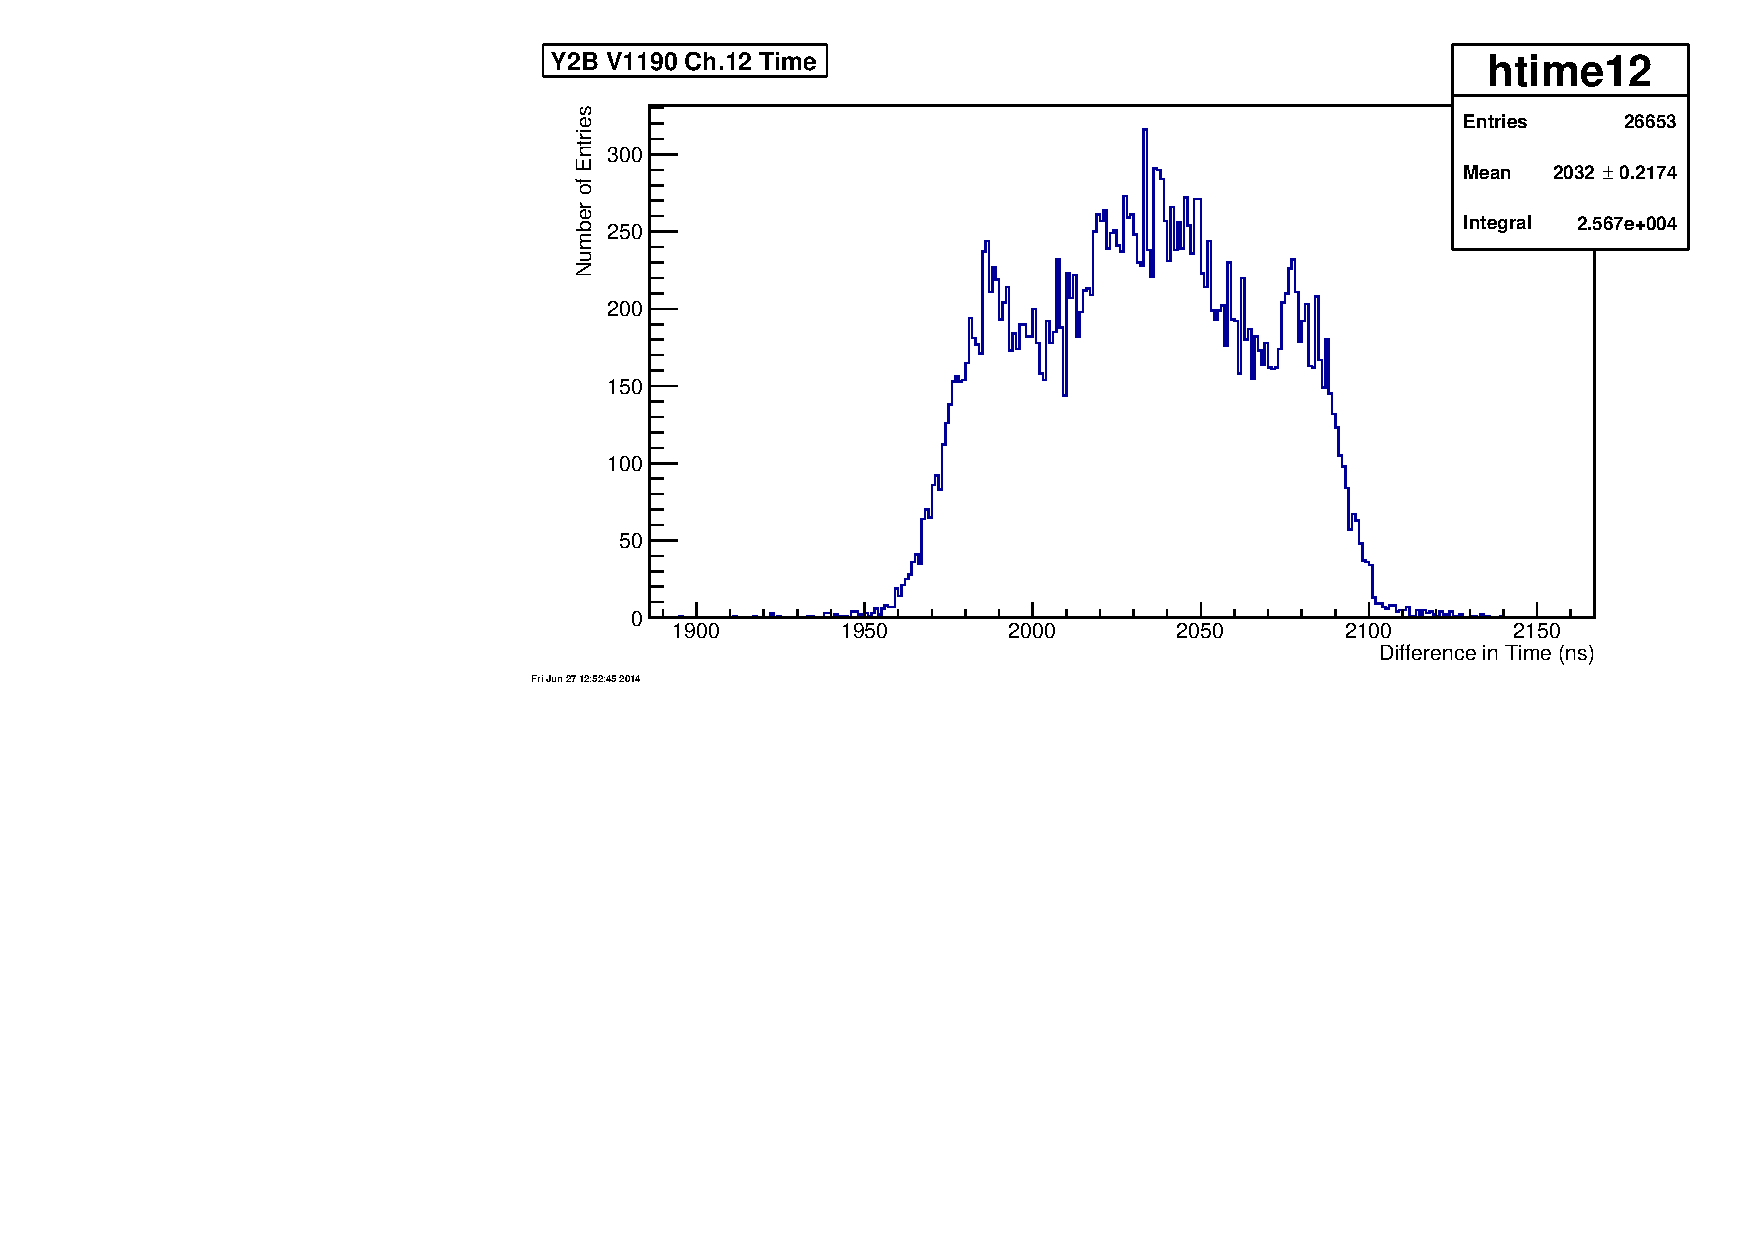
\includegraphics[width=\columnwidth]{run00480_htime12}%
\caption{Raw (uncalibrated) timing spectrum for cathode position signal Y2B.  The range of the timing signal is approximately 150\,ns.  This corresponds to a detector area of 60\,mm, indicating that some of the events are detected outside of the 54\,mm-wide fudicial area of the detector.}%
\label{htime}%
\end{figure}

%\ldots it was suggested that using two detectors may allow ray-tracing of the incident particles.  